%!TEX root = ../main.tex

Nesta seção serão apresentados os resultados parciais obtidos no teste de modelos baseados em algumas das arquiteturas selecionadas para o escopo deste trabalho. As Seções \ref{sec:lenet} e \ref{sec:alexnet} demonstram os resultados obtidos pelos melhores modelos encontrados com as arquiteturas LeNet e AlexNet, respectivamente. O treinamento destas CNNs foi realizado utilizando os recursos computacionais de um servidor, disponível no LSI, dedicado especialmente para tarefas de DL, o qual possui um processador Intel Core i7 com 16 GB de RAM e duas placas gráficas com 11 GB de memória cada, ajudando no processamento dos algoritmos de aprendizado.

Após a etapa de treino, foram realizados os testes para aferir os modelos no tocante às métricas de desempenho para o conjunto de testes. Nesta etapa, percebeu-se que alguns modelos tornaram-se degenerados e acabaram prevendo apenas uma das classes. Duas hipóteses podem justificar a ocorrência desse problema: o ReLU \emph{dying problem}, quando a função de ativação ReLU foi utilizada; ou a tendência a permanência em mínimos locais durante o treinamento do modelo. Todas as CNNs que manifestaram este comportamento no conjunto de testes tiveram seus resultados descartados, pois as métricas obtidas não refletiam o aprendizado do problema considerado.


\subsection{Resultados Obtidos com a CNN LeNet}
\label{sec:lenet}

A primeira fase do treinamento dos modelos foi conduzida utilizando a arquitetura LeNet. Nesta fase, foi realizada uma busca em \emph{grid} por todos os hiperparâmetros previamente definidos, conforme Seção \ref{sec:modelos}, gerando um total de $36$ modelos a serem treinados e testados. Para estes modelos, excluindo aqueles que se tornaram degenerados, utilizou-se a métrica \emph{F-score} como referência para um melhor desempenho. Em relação aos três otimizadores considerados, os modelos dispostos na Tabela \ref{tab:lenet} foram identificados como tendo melhor desempenho para a tarefa em questão.

\begin{table}[h!]
\centering
\caption{Detalhamento dos melhores modelos obtidos com a arquitetura LeNet, organizados de forma decrescente considerando o valor de acurácia.}
\label{tab:lenet}
\begin{tabular}{ccccc}
\toprule
\textbf{Otimizador} & \textbf{\emph{Patience}}  & \textbf{Função de Ativação} & \textbf{Acurácia} & \textbf{F-Score} \\
\midrule
RMSprop & 5 & \emph{Leaky} ReLU & $0.9865$ & $0.9755$ \\
SGD & 5 & ELU & $0.9787$ & $0.9619$ \\
Adam & 10 & ReLU & $0.9366$ & $0.8974$ \\
\bottomrule
\end{tabular}
\end{table}


Os gráficos da Figura \ref{fig:treinamento-lenet} denotam o histórico da perda (\emph{loss}) e acurácia para o conjunto de treinamento e validação destas redes. Nota-se que nenhuma delas chegou ao limite máximo de épocas possíveis, interrompendo o aprendizado por meio de \emph{early stopping}.


\begin{figure}[H]
	\centering
	\caption{Histórico de \emph{loss} e acurácia durante o treinamento dos melhores modelos obtidos com a arquitetura LeNet.}
	\subfloat[\emph{Loss} durante treinamento do melhor modelo com RMSprop.\label{subfig:lenet-rmsprop-loss}]{%
	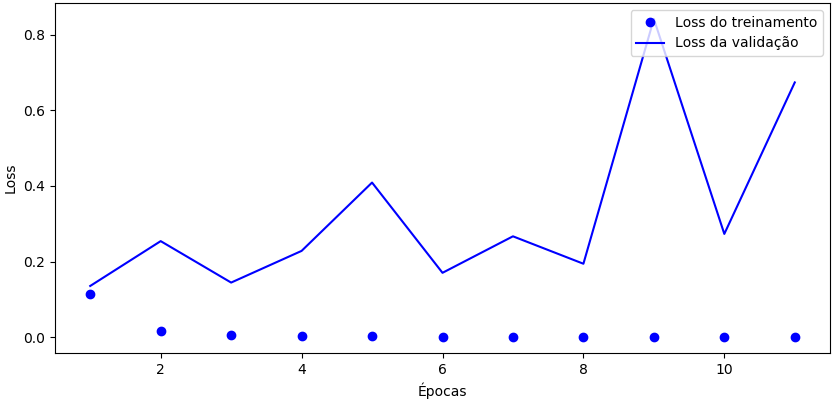
\includegraphics[width=0.45\textwidth]{imgs/lenet-rmsprop-loss}
	}
	\subfloat[Acurácia durante treinamento do melhor modelo com RMSprop.\label{subfig:lenet-rmsprop-acc}]{%
	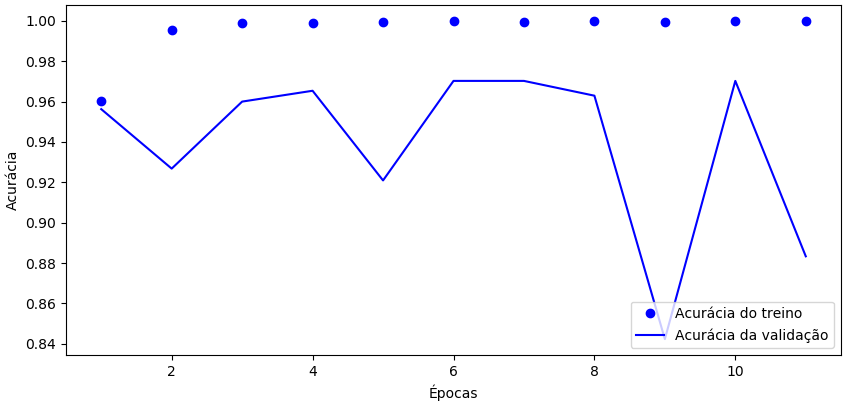
\includegraphics[width=0.45\textwidth]{imgs/lenet-rmsprop-acc}
	}
	\hfill
	\subfloat[\emph{Loss} durante treinamento do melhor modelo com SGD.\label{subfig:lenet-sgd-loss}]{%
	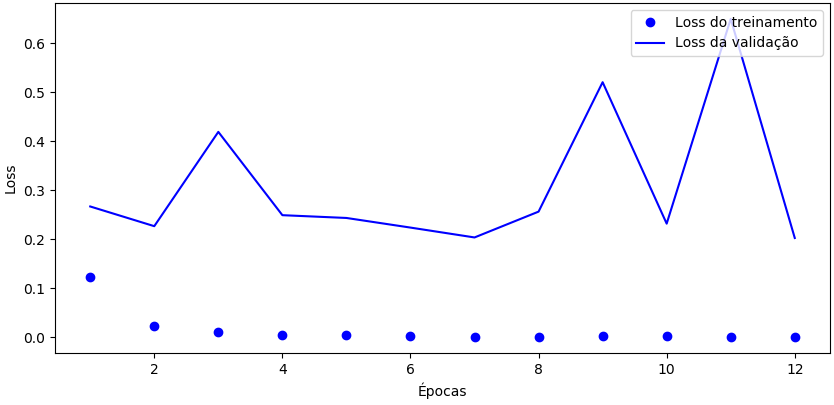
\includegraphics[width=0.45\textwidth]{imgs/lenet-sgd-loss}
	}
	\subfloat[Acurácia durante treinamento do melhor modelo com SGD.\label{subfig:lenet-sgd-acc}]{%
	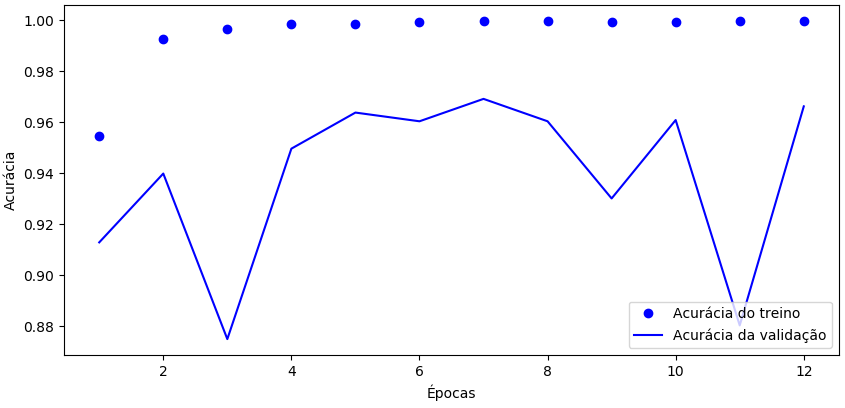
\includegraphics[width=0.45\textwidth]{imgs/lenet-sgd-acc}
	}
	\hfill
	\subfloat[\emph{Loss} durante treinamento do melhor modelo com Adam.\label{subfig:lenet-adam-loss}]{%
	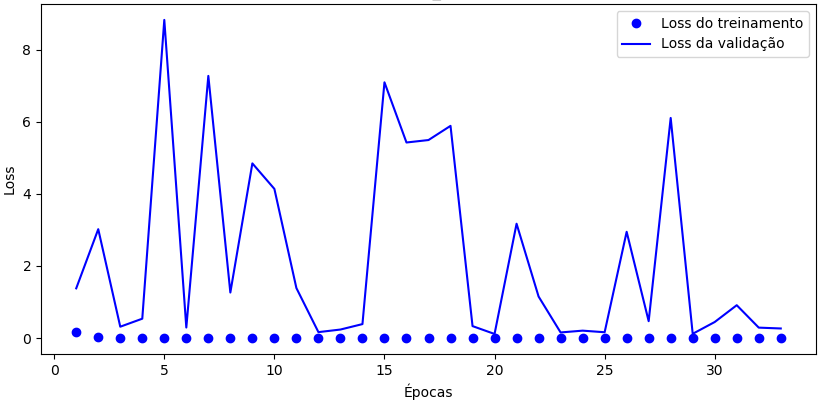
\includegraphics[width=0.45\textwidth]{imgs/lenet-adam-loss}
	}
	\subfloat[Acurácia durante treinamento do melhor modelo com Adam.\label{subfig:lenet-adam-acc}]{%
	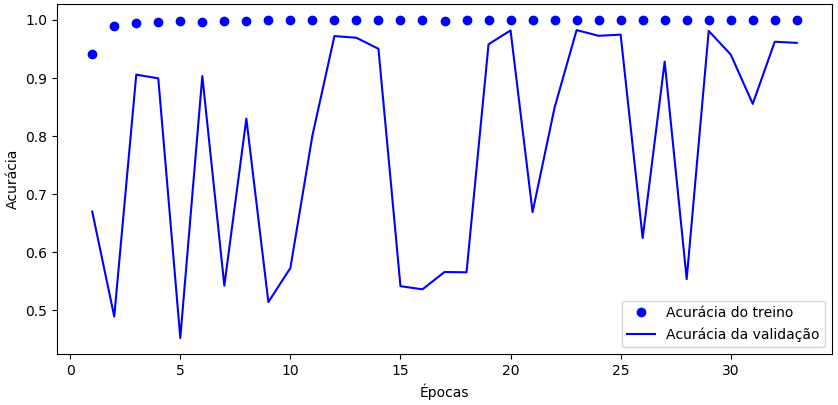
\includegraphics[width=0.45\textwidth]{imgs/lenet-adam-acc}
	}
	\label{fig:treinamento-lenet}
\end{figure}

Examinando mais atentamente o desempenho destas redes no conjunto de testes, tem-se, então, as matrizes de confusão mostradas na Figura \ref{fig:matrizes-lenet}. Nestas matrizes, a soma das linhas representam a quantidade de assinaturas previstas para cada classe pelo modelo em questão, enquanto a soma das colunas denotam a quantidade de assinaturas existentes em cada classe.

\begin{figure}[H]
	\centering
	\caption{Matrizes de confusão dos melhores modelos obtidos com a arquitetura LeNet.}\label{fig:matrizes-lenet}
	\subfloat[Abordagem 1\label{subfig:matriz-approach1-lenet}]{%
	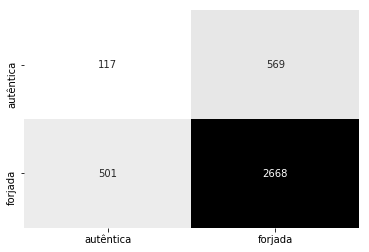
\includegraphics[width=0.5\textwidth]{imgs/matriz-approach1-lenet}
	}
	\subfloat[Abordagem 2\label{subfig:matriz-approach2-lenet}]{%
	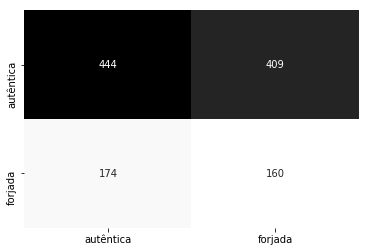
\includegraphics[width=0.5\textwidth]{imgs/matriz-approach2-lenet}
	}
	\hfill
	\subfloat[Abordagem 3\label{subfig:matriz-approach1-lenet}]{%
	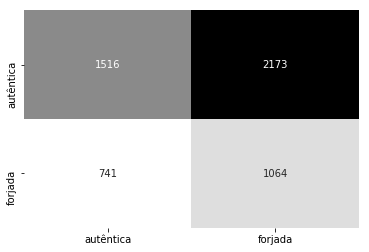
\includegraphics[width=0.5\textwidth]{imgs/matriz-approach3-lenet}
	}
\end{figure}

%%%% ARGUMENTAÇÃO

Para esta arquitetura, é possível visualizar que os melhores modelos foram aqueles que possuíram o menor valor de \emph{patience}. Isso revela que houve uma oscilação no treinamento, de modo que o aprendizado de característica sobre o problema foi instável, resultando em uma parada precoce. Para contornar este efeito, pode ser necessário buscar ajustes de parâmetros (\emph{fine-tuning}) ou também avaliar outras arquiteturas nesta tarefa, nas quais este efeito é minimizado.

No geral, o desempenho obtido com as redes LeNet ainda não foram suficientemente bons para a tarefa considerada. Embora a acurácia denote valores altos para a primeira abordagem ($0.7224$), precisa-se relembrar que isto é mais predominantemente decorrente do desbalanceamento do \emph{dataset} do que da qualidade do modelo em si, conforme revela o \emph{F-Score} associado ($0.1794$). As matrizes de confusão ilustradas na Figura \ref{fig:matrizes-lenet} denotam uma diagonal principal ainda pouco densa, sugerindo que melhorias na tarefa ainda são necessárias. Neste ponto, tem-se os resultados da Abordagem 2 como sendo melhores para a tarefa considerada.



\subsection{Resultados Obtidos com a CNN AlexNet}
\label{sec:alexnet}
 %% Trabalhar aqui

 Para a AlexNet, assim como para a CNN anterior, foi realizada uma busca em \emph{grid} com os hiperparâmetros selecionados anteriormente, com vistas a obter os melhores modelos para cada abordagem de separação de dados, gerando assim, mais 108 modelos a serem avaliados quanto as suas métricas de desempenho.

 Mais uma vez considerando a métrica de \emph{F-score}, foram selecionados os melhores modelos e estes encontram-se listados na Tabela \ref{tab:alexnet}.

 \begin{table}[h!]
 \centering
 \caption{Detalhamento dos melhores modelos obtidos com a arquitetura AlexNet, organizados de forma decrescente considerando o valor de Acurácia.}
 \label{tab:alexnet}
 \begin{tabular}{cccccc}
 \toprule
 \textbf{Conjunto} & \textbf{Otimizador} & \textbf{\emph{Patience}}  & \textbf{Função de Ativação} & \textbf{Acurácia} & \textbf{F-Score} \\
 \midrule
 Abordagem 2 & SGD & 5 & \emph{Leaky} ReLU & $0.5282$ & $0.6349$ \\
 Abordagem 3 & Adam & 15 & SELU & $0.4456$ & $0.5524$ \\
 Abordagem 1 & RMSprop & 5 & ReLU & $0.1844$ & $0.2765$ \\
 \bottomrule
 \end{tabular}
\end{table}


\begin{figure}[H]
	\centering
	\caption{Histórico de \emph{loss} e acurácia durante o treinamento dos melhores modelos obtidos com a arquitetura AlexNet.}
	\subfloat[\emph{Loss} durante treinamento com a Abordagem 1\label{subfig:approach1-alexnet-loss}]{%
	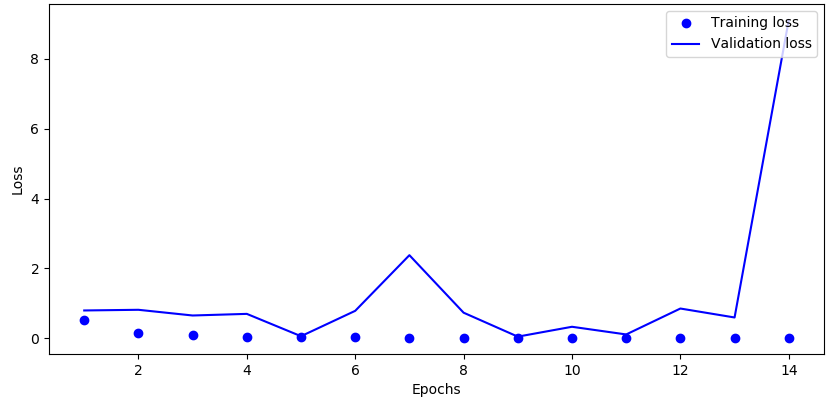
\includegraphics[width=0.45\textwidth]{imgs/approach1-alexnet-rmsprop-5-relu-loss}
	}
	\subfloat[Acurácia durante treinamento com a Abordagem 1\label{subfig:approach1-alexnet-acc}]{%
	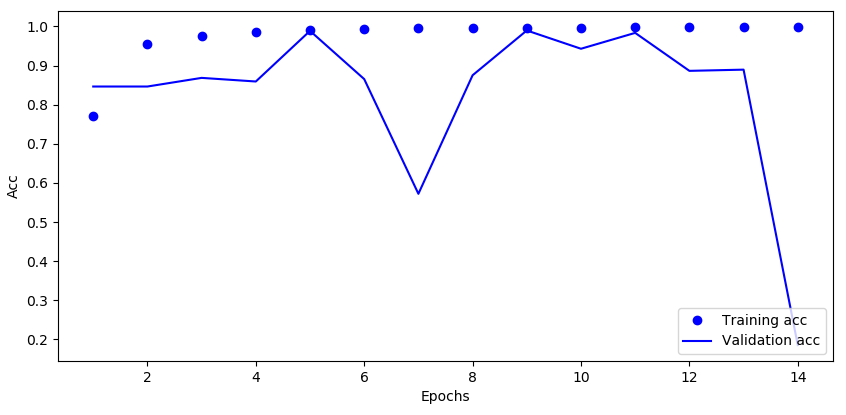
\includegraphics[width=0.45\textwidth]{imgs/approach1-alexnet-rmsprop-5-relu-acc}
	}
	\hfill
	\subfloat[\emph{Loss} durante treinamento com a Abordagem 2\label{subfig:approach2-alexnet-loss}]{%
	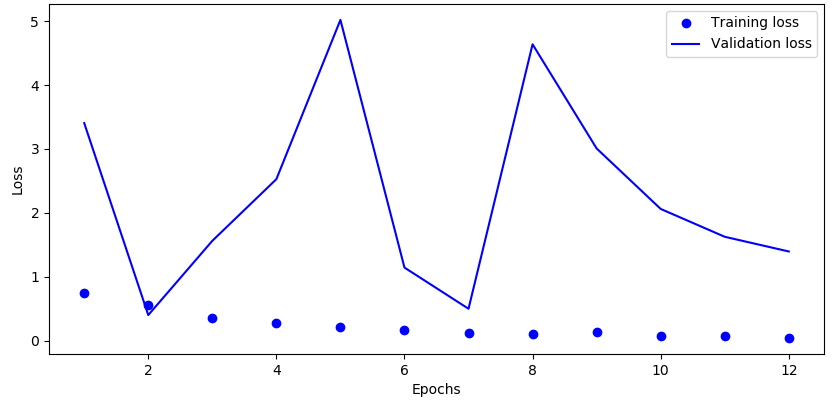
\includegraphics[width=0.45\textwidth]{imgs/approach2-alexnet-sgd-5-lrelu-loss}
	}
	\subfloat[Acurácia durante treinamento com a Abordagem 2\label{subfig:approach2-alexnet-acc}]{%
	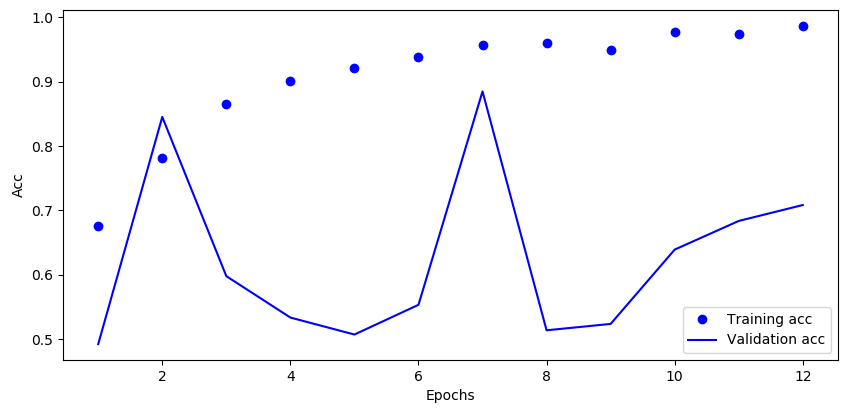
\includegraphics[width=0.45\textwidth]{imgs/approach2-alexnet-sgd-5-lrelu-acc}
	}
	\hfill
	\subfloat[\emph{Loss} durante treinamento com a Abordagem 3\label{subfig:approach3-alexnet-loss}]{%
	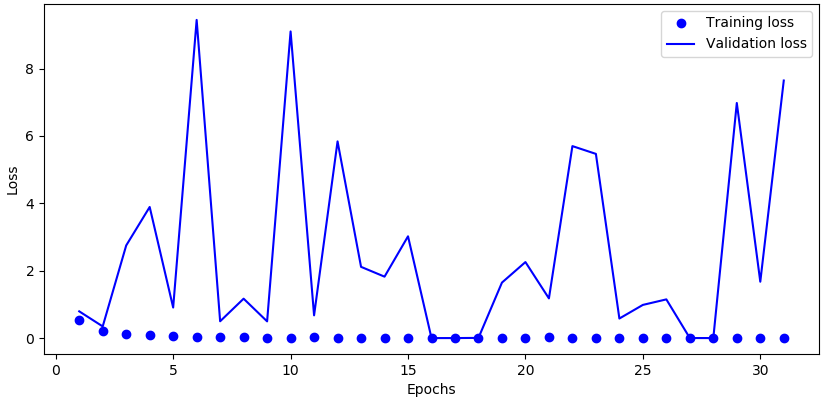
\includegraphics[width=0.45\textwidth]{imgs/approach3-alexnet-adam-15-selu-loss}
	}
	\subfloat[Acurácia durante treinamento com a Abordagem 3\label{subfig:approach3-alexnet-acc}]{%
	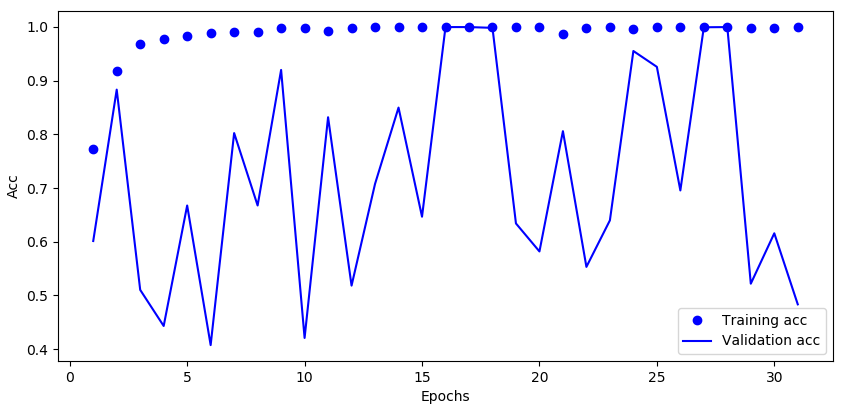
\includegraphics[width=0.45\textwidth]{imgs/approach3-alexnet-adam-15-selu-acc}
	}
	\label{fig:treinamento-alexnet}
\end{figure}


\begin{figure}[h!]
	\centering
	\caption{Matrizes de confusão dos melhores modelos obtidos com a arquitetura AlexNet.}
	\subfloat[Abordagem 1\label{subfig:matriz-approach1-alexnet}]{%
	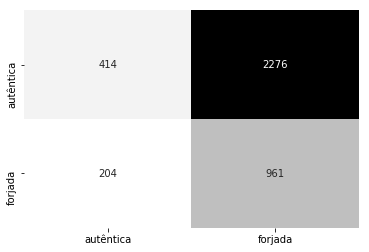
\includegraphics[width=0.5\textwidth]{imgs/matriz-approach1-alexnet}
	}
	\subfloat[Abordagem 2\label{subfig:matriz-approach2-alexnet}]{%
	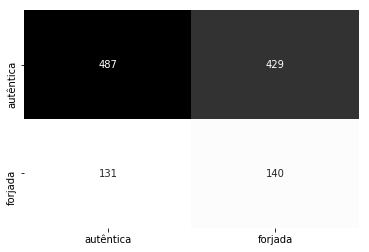
\includegraphics[width=0.5\textwidth]{imgs/matriz-approach2-alexnet}
	}
	\hfill
	\subfloat[Abordagem 3\label{subfig:matriz-approach1-alexnet}]{%
	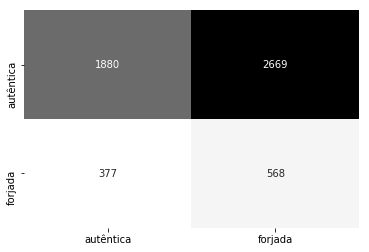
\includegraphics[width=0.5\textwidth]{imgs/matriz-approach3-alexnet}
	}
	\label{fig:matrizes-alexnet}
\end{figure}
